%% chapter 4 dataset, network structure, experiment and result
\chapter{实验与结果}
\label{cha:experiment}
\section{login和register模块}
利用注册登录模块机型账户管理,每个用户登录之后都能看到自己相关的页面。如自己参与了那些产品的开发或者测试等等。
\begin{figure}[h]
	\centering
	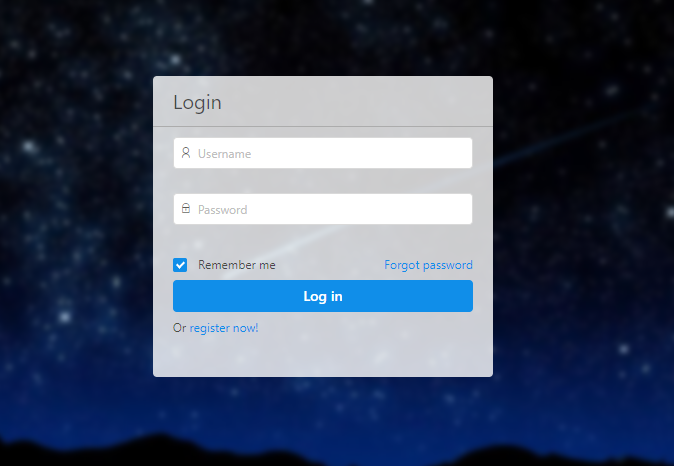
\includegraphics[width=0.5\textwidth]{image/result/login.png}
	\caption{登录模块}
	\label{fig:login}
\end{figure}
\begin{figure}[h]
	\centering
	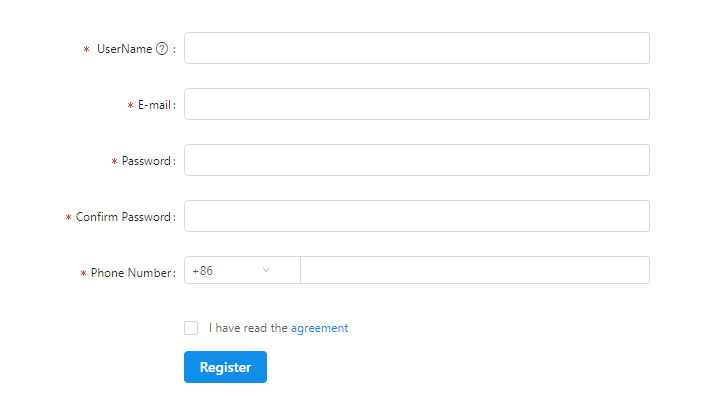
\includegraphics[width=0.8\textwidth]{image/result/register.png}
	\caption{注册模块}
	\label{fig:register}
\end{figure}
\section{newProduct和newVersion模块}
新建产品和新建版本模块有些相似,因为新建产品的时候会新建产品的第一个版本,也需要上传资源包
\begin{figure}[h]
	\centering
	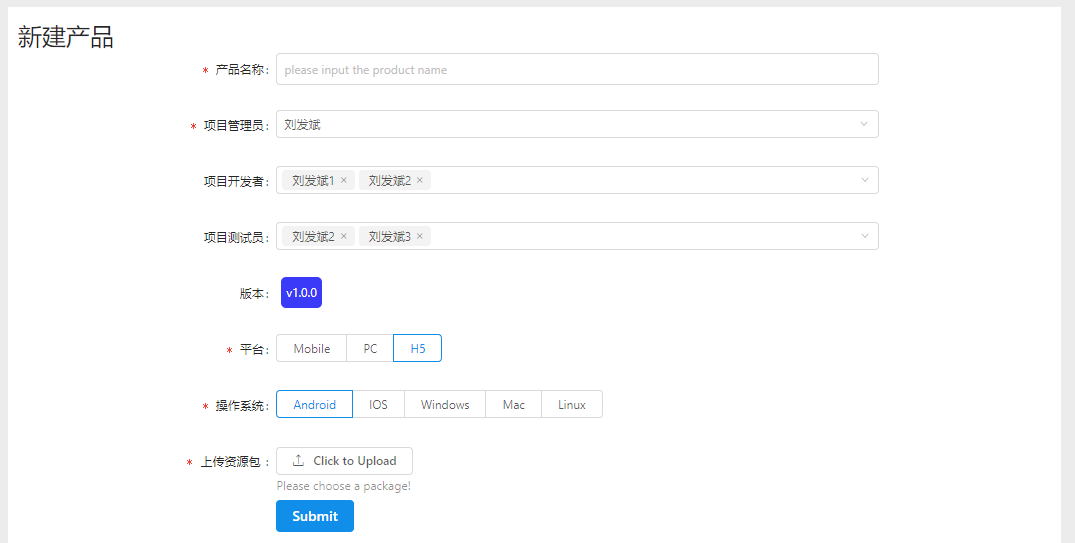
\includegraphics[width=0.8\textwidth]{image/result/product.png}
	\caption{新建产品}
	\label{fig:newProduct}
\end{figure}
\begin{figure}[h]
	\centering
	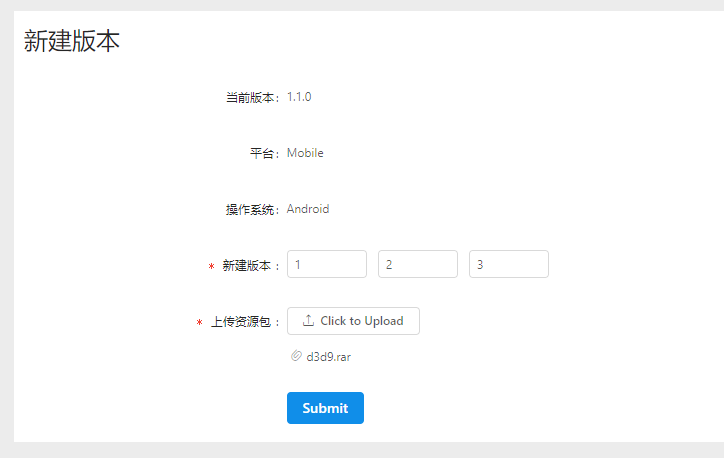
\includegraphics[width=0.8\textwidth]{image/result/version.png}
	\caption{新建版本}
	\label{fig:newVersion}
\end{figure}
\section{数据展示模块}
\subsection{侧边栏}
如图4-5
\begin{figure}[h]
	\centering
	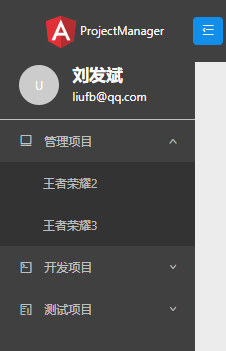
\includegraphics[width=0.2\textwidth]{image/result/sidebar.png}
	\caption{侧边栏}
	\label{fig:side}
\end{figure}
\subsection{产品列表}
前端根据用户的id查询与用户相关的所有产品列表并返回
\begin{figure}[h]
	\centering
	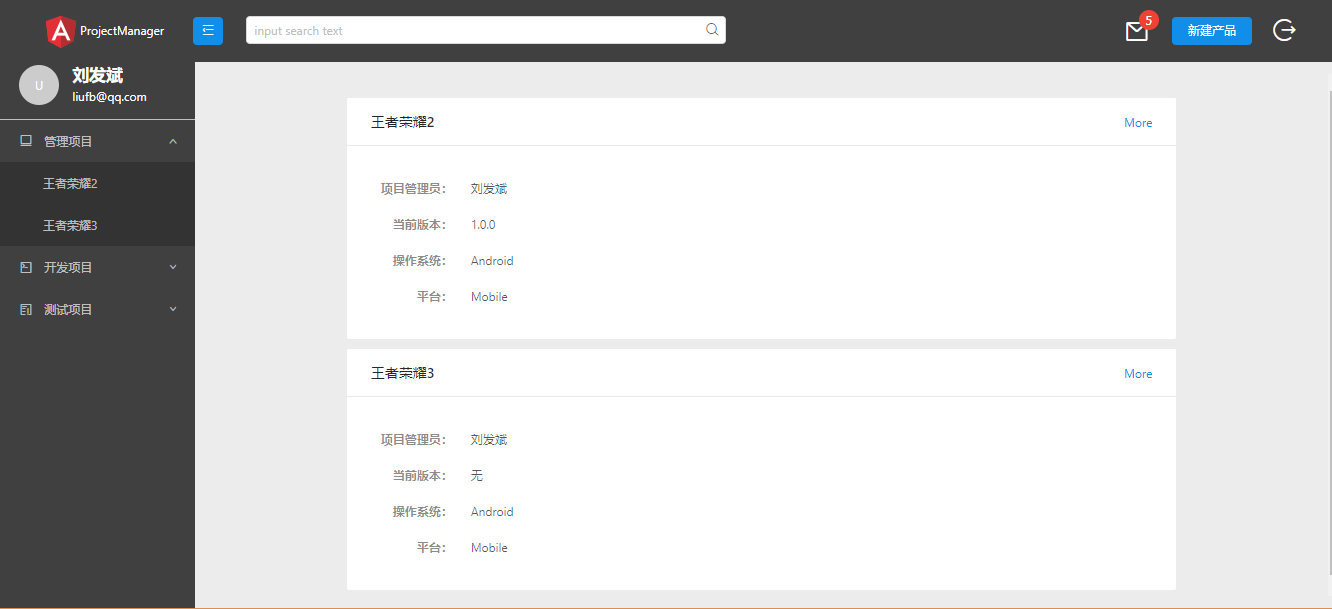
\includegraphics[width=\textwidth]{image/result/list.png}
	\caption{产品列表}
	\label{fig:list}
\end{figure}
\subsection{产品详情}
产品详情包括:产品信息、成员列表、版本流程、产品管理员的审核页面。其实产品详情页面是一个页面,产品信息,成员列表等都是利用tab组件来进行切换视图的。产品详情包括产品的信息和版本信息,成员分组列表,版本流程包括版本的回滚以及根据状态码显示的状态流程。提测审核页面只有产品管理员可以看到,这个需要前端设置权限。
\begin{figure}[h]
	\centering
	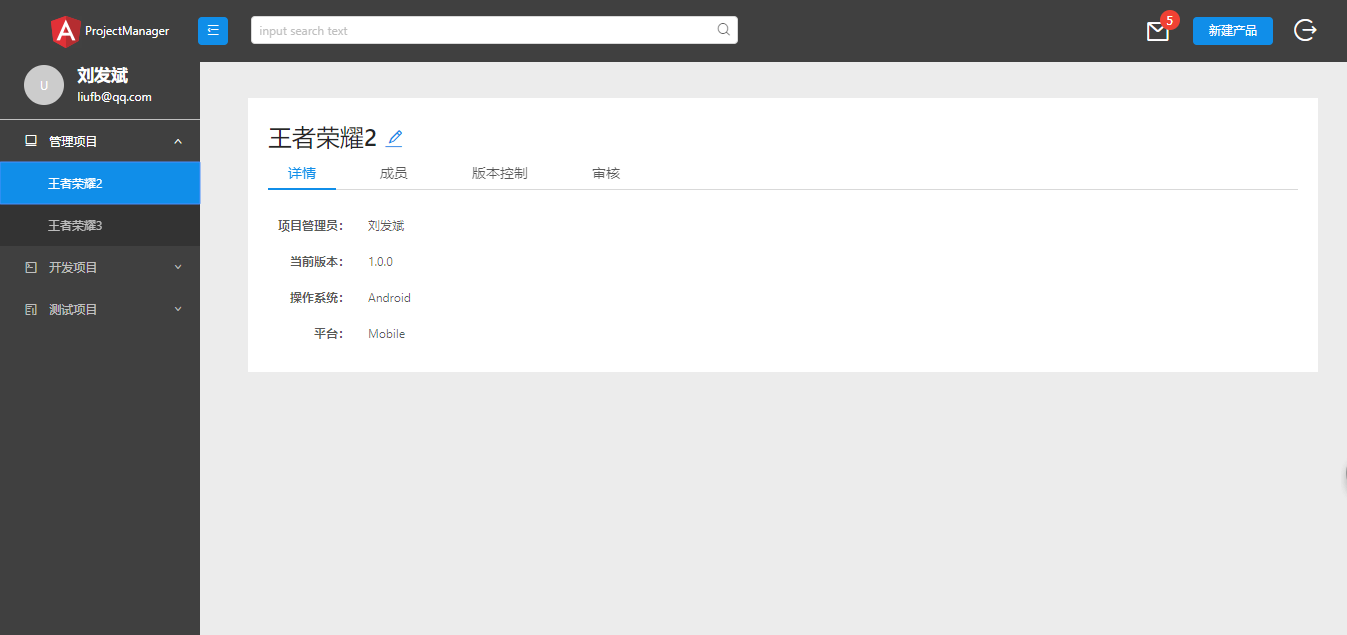
\includegraphics[width=\textwidth]{image/result/detail.png}
	
	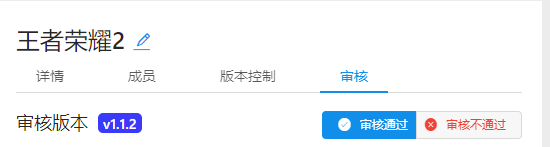
\includegraphics[width=\textwidth]{image/result/check.png}
	
	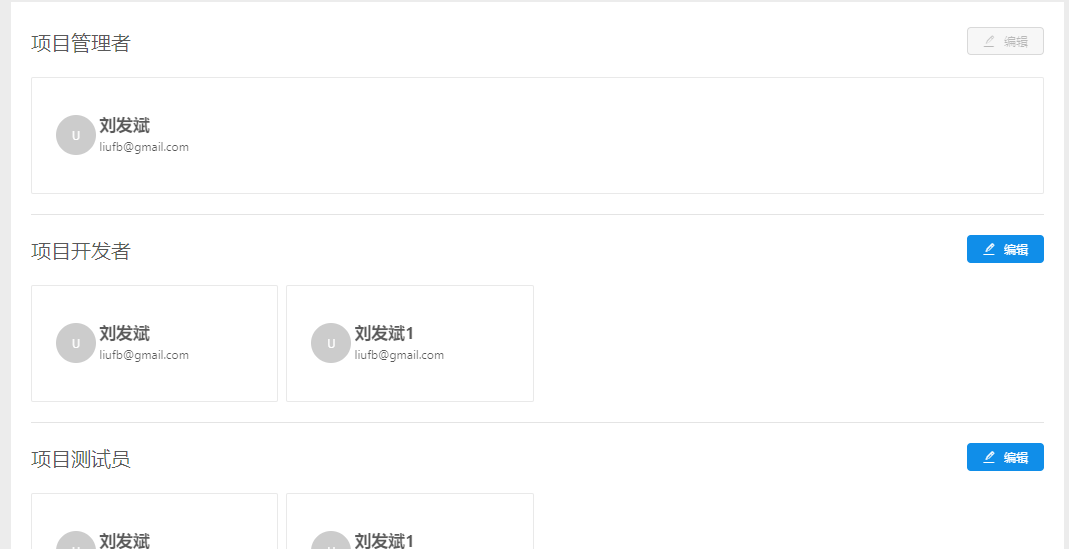
\includegraphics[width=\textwidth]{image/result/member.png}
	
	\includegraphics[width=\textwidth]{image/result/versionflow.png}
	\caption{产品详情}
	\label{fig:detail}
\end{figure}
系统信息列表显示的是跟用户相关的变动通知,可以从顶部栏的信封图标入口进入
\begin{figure}[h]
	\centering
	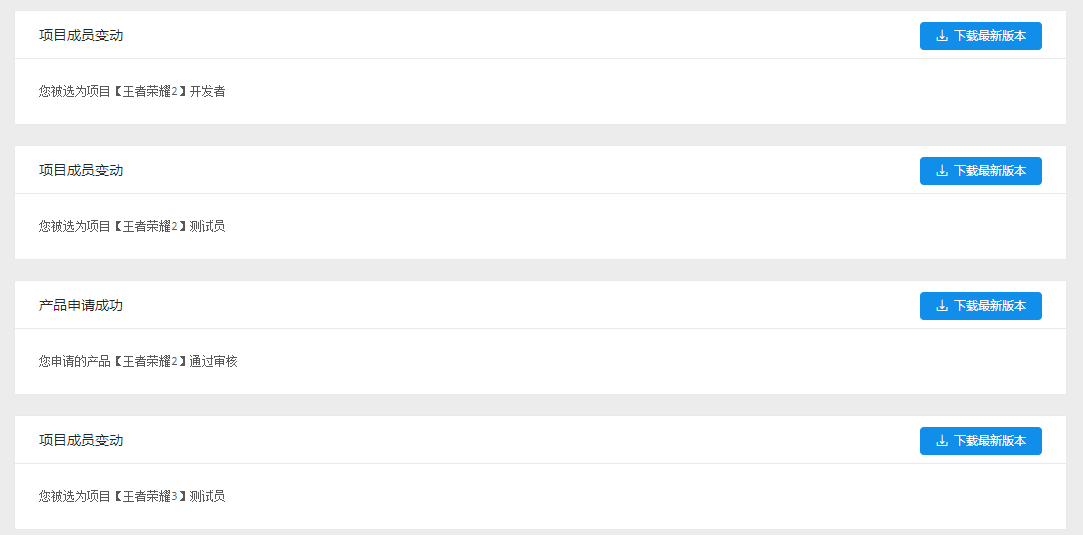
\includegraphics[width=0.8\textwidth]{image/result/message.png}
	\caption{系统信息列表}
	\label{fig:message}
\end{figure}
\section{后台相关的业务流程}
\begin{figure}[h]
	\centering
	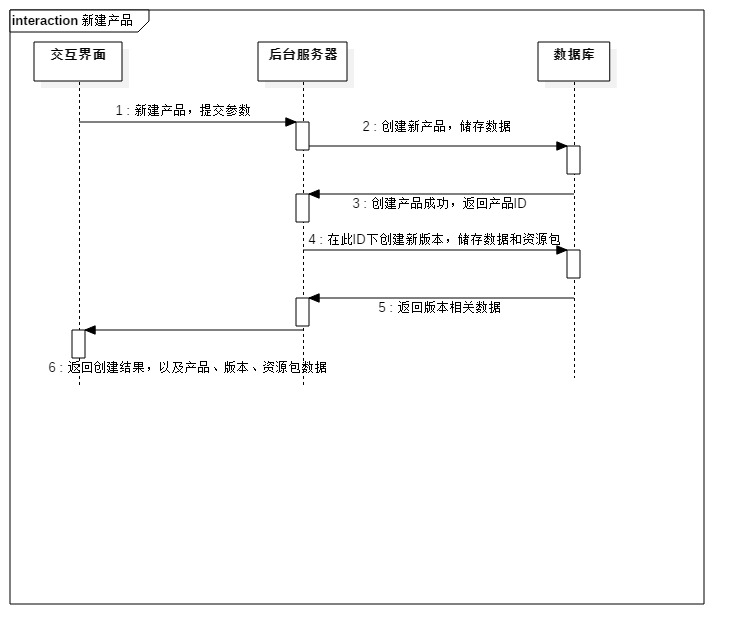
\includegraphics[width=\textwidth]{image/UML/newProduct.png}
	
	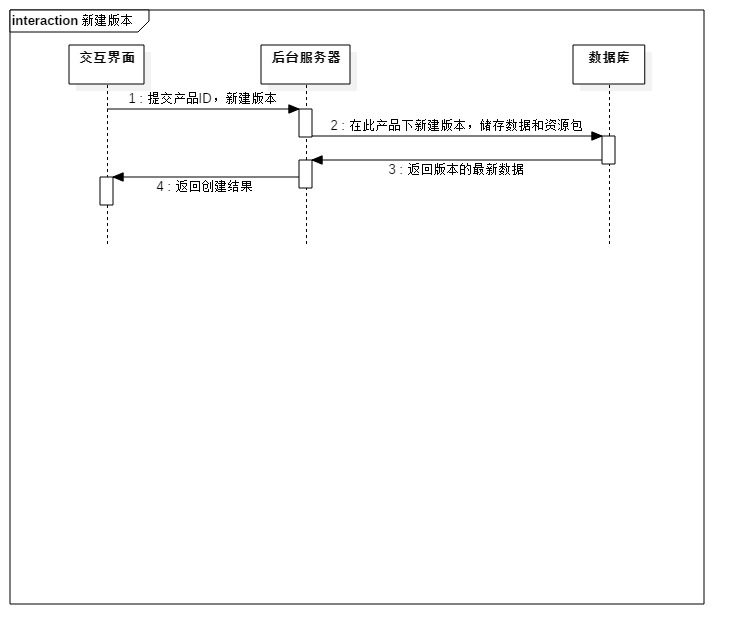
\includegraphics[width=\textwidth]{image/UML/newVersion.png}
	
	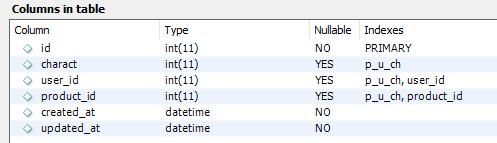
\includegraphics[width=\textwidth]{image/UML/member.png}
	
	\includegraphics[width=\textwidth]{image/UML/versionflow.png}
	\caption{产品详情}
	\label{fig:detail}
\end{figure}